% 2015-05-21 - Emerson Ribeiro de Mello - mello@ifsc.edu.br
% \documentclass[handout,xcolor=pdftex,dvipsnames,table]{beamer}
\documentclass{beamer}

\usepackage[utf8]{inputenc}
\usepackage[T1]{fontenc}
\usepackage[portuguese]{babel}

% usando tema personalizado. 
% arquivo beamerthemeIFSC.sty deve estar no mesmo diretório do .tex
\usepackage{beamerthemeIFSC}
\usepackage{tikz}
\usepackage{xargs}
\usepackage{amsmath}
\usepackage{mathtools}
\usepackage{soul} %fazer texto tachado
\usepackage{epigraph}
\usepackage[colorinlistoftodos,prependcaption,textsize=tiny]{todonotes}


\usepackage{xargs}
%
\newcommandx{\unsure}[2][1=]{\todo[linecolor=red,backgroundcolor=red!25,bordercolor=red,#1]{#2}}
\newcommandx{\info}[2][1=]{\todo[linecolor=OliveGreen,backgroundcolor=OliveGreen!25,bordercolor=OliveGreen,#1]{#2}}
%

\hypersetup{pdfstartview={Fit},pdftitle={\@title},
 	pdfsubject={IFBA},pdfauthor={\@author}
}

\hyphenation{ob-je-ti-vo}


%%%%%%%%%%%%%%%%%%%%%%%%%%%%%%%%%%%%%%%%%%%%


\title{Conhecendo o \LaTeX}
\subtitle{mudando a perspectiva}
\author{Ícaro Jerry}
\date{29 de março de 2017}
\institute{Instituto Federal da Bahia\\
campus Salvador\\
\url{icarojerry@ifba.edu.br}
}



%%%%%%%%%%%%%%%%%%%%%%%%%%%%%%%%%%%%%%%%%%%%

\begin{document}

\begin{frame}[t]
	\maketitle
\end{frame}

% Descomente as linhas abaixo se desejar colocar um sumário de todas as seções
\begin{frame}[t]{Agenda}
\tableofcontents
\end{frame}

% O trecho de código abaixo serve para sobrescrever regras do template
\def\sectionname{}
\def\insertsectionnumber{}
\def\subsectionname{}
\def\insertsubsectionnumber{}

\AtBeginSection{\frame{\sectionpage}\addtocounter{framenumber}{-1}}


\AtBeginSubsection{\frame{\subsectionpage}\addtocounter{framenumber}{-1} }
\AtBeginSubsubsection{\frame{\subsubsectionpage}\addtocounter{framenumber}{-1} }



%%%%%%%%%%%%%%%%%%%%%%%%%%%%%%%%%%%%%%%%%%%%
% Inicio do documento
%%%%%%%%%%%%%%%%%%%%%%%%%%%%%%%%%%%%%%%%%%%%

\begin{frame}{Quem sou eu?}
    \begin{itemize}
        \item Meu nome é Ícaro Jerry,
        \item Sou aluno dinossauro de ADS (IFBA),
        \item Entusiasta de Tecnologias Livres $\backslash$o/
        \item Membro e Colaborador do OPAI e KDE
        \item \textbf{Contatos}:        
        \begin{itemize}
            \item \textbf{E-mail}: icarojerry at $\{$gmail.com || ifba.edu.br$\}$
            \item \textbf{LinkedIn}: linkedin.com/in/icarojerry
            \item \textbf{GitHub}: github.com/IcaroJerry/
        \end{itemize}
    \end{itemize}
\end{frame}
%

\section{Introdução}
\begin{frame}{Primeiro, a briga da pronuncia...}
    \begin{itemize}
        \item  O nome \TeX é composto por três letras gregas:
        \begin{itemize}
            \item $\tau$ (tau)
            \item $\epsilon$ (épsilon)
            \item $\chi$ (chi, pronunciado \textit{qui})
        \end{itemize}
        \item Daí vem $\tau$$\epsilon$$\chi$, ou téc
        \item Finalmente, \LaTeX, ou \textit{latéc} (em inglês ficaria lei-téc)
        \item Porém, não é bem isso que acontece... então fique a vontade para chamar como se sentir mais confortável
    \end{itemize}
    

\end{frame}
%

\begin{frame}{O que é o \LaTeX?}
    \begin{itemize}
        \item Em poucas palavras:  \LaTeX é um sistema tipográfico de alta qualidade que provê funcionalidades focadas na produção de textos
        \item  Pode ser utilizada para redação de qualquer documento: desde uma simples carta até livros completos, desde trabalhos de faculdade até artigos científicos, desde relatórios até apresentações...
    \end{itemize}
\end{frame}
%

\begin{frame}{E para que serve?}
    \begin{itemize}
        \item O \LaTeX é um grande aliado para pessoas que precisam produzir textos acadêmicos e científicos
        \item É geralmente utilizado principalmente por profissionais do meio acadêmico das áreas de Ciências Exatas
        \item Ideal para qualquer pessoa que queria otimizar a produção de textos e economizar tempo
        \item Facilita diversas atividades comuns na construção de um texto, tais como, uso de fórmulas e equações matemáticas; criação de tabelas e imagens; e gerência das referências e citações
    \end{itemize}
\end{frame}

\begin{frame}{Contexto Histórico}
    \begin{description}
        \item[1977] Donald E. Knuth criou um programa \TeX com linguagem própria para processar textos e fórmulas matemáticas eletronicamente com o objetivo de aumentar a qualidade de impressão naquela época
        \item[1982] Lançada a primeira versão estável do \TeX
        \item[1985] Leslie Lamport criou um conjunto de macros chamada \LaTeX para simplificar o uso do \TeX
        \item[]
        \item[] Oficial do projeto: \textit{\url{https://www.latex-project.org/}}
    \end{description}
    
    
\end{frame}
%

\begin{frame}{Mudando a Perspectiva}
    \begin{itemize}
        \item Processadores WYSIWYG (\textbf{W}hat \textbf{Y}ou \textbf{S}ee \textbf{I}s \textbf{W}hat \textbf{Y}ou \textbf{G}et)
        \begin{itemize}
            \item Exemplos: LibreOffice, MS Word, Corel WordPerfect...
        \end{itemize}
        \item[]
        \item Processadores WYSIWYM (\textbf{W}hat \textbf{Y}ou \textbf{S}ee \textbf{I}s \textbf{W}hat \textbf{Y}ou \textbf{M}ean)
        \begin{itemize}
            \item Exemplos: HTML, QML, \LaTeX...
        \end{itemize}
    \end{itemize}
\end{frame}
%

\begin{frame}{Pontos Negativos}
    \begin{itemize}
        \item Curva de aprendizado
        \item Complexidade de criar novos \textit{layouts} ou alterá-los
        \item Configuração do ambiente as vezes pode se tornar complicada*
        \item Procedimento de processamento (compilação) não é trivial,\\ inclusive em alguns editores
    \end{itemize}
\end{frame}

\begin{frame}{Pontos Positivo}
    \begin{itemize}
        \item São muitos!
        \item Tanto o \LaTeX e o \TeX  são \textbf{Open Source}
        \item Existem diversas ferramentas auxiliares
        \item Permitem criar textos com alta qualidade tipográfica
        \item Os textos e seus elementos ficam com aparência profissional
        \item Diversos \textit{layouts} e \textit{templates} prontos
        \item Estruturas tipográficas complexas (bibliografia, tabela de
        conteúdo, citações) podem ser criadas facilmente
        \item Numeração e citação automáticas
        \item Evitam erro de \textit{layouts}
        
    \end{itemize}
\end{frame}
\begin{frame}{Pontos Positivo}
    \begin{itemize}
        \item Pacotes para gerar vários tipos de documentos
        \begin{itemize}
            \item Artigos
            \item Relatórios
            \item Livros
            \item Slides
            \item Poster
            \item Apresentação
        \end{itemize}
        
        \item Foco nos comandos e não na estrutura
        \item Economia de tempo e foco no mais importante (o texto)
        \item Troca de \textit{layout} simples, as vezes com uma \textbf{única} palavra
        \item Possibilidade de versionamento
        \item E muitos outros...
    \end{itemize}
\end{frame}


\section{Instalando o \LaTeX}
\begin{frame}{Requisitos}
    \begin{itemize}
        \item Para poder utilizar \LaTeX basicamente você precisa de:
        \begin{enumerate}
            \item Editor de texto
            \item Compilador
        \end{enumerate}

        \item O arquivo fonte de um texto em \LaTeX é basicamente:
        \begin{itemize}
            \item texto
            \item \textit{tags}
        \end{itemize}
    \item No final, o arquivo gerado é (normalmente): .ps ou .pdf
    \item Porém, existem ferramentas que auxiliam nesse processo
    \end{itemize}
\end{frame}

\begin{frame}{Editor \& Compilador}
    \begin{itemize}
        \item O arquivo fonte do texto \LaTeX pode ser escritos em um editor de texto simples ou específico
        
        \item Os específicos trazem algumas vantagens como:
        \begin{itemize}
            \item compilação automática
            \item \textit{highlight}
            \item \textit{templates}
            \item \textit{autocomplete}
            \item pré-visualização instantânea
            \item dentre outras
        \end{itemize}
    \end{itemize}
\end{frame}

\begin{frame}{Ferramentas de auxílio}
    
    \begin{itemize}
        \item Alguns editores específicos para \LaTeX são:
        \begin{itemize}
            \item Desktop:
            \begin{itemize}
                \item TexStudio
                \item TeXnicCenter
                \item TexMaker
                \item Kile
            \end{itemize}
            \item Web:
                \begin{itemize}
                \item Share\LaTeX
                \item Papeeria
                \item Overleaf
                \item Datazar
            \end{itemize}
        \end{itemize}
        \item Os editores Desktop podem ser mais personalizados e eficientes 
        \item Já os editores Web resolvem a configuração do ambiente \LaTeX
         
    \end{itemize}
\end{frame}

%Linux
\begin{frame}{Instalação em Ambientes Desktop}
    \begin{itemize}
    \item Linux
    \begin{itemize}
        \item Vai depender muito da distribuição
        \item Geralmente, busca pelo pacote \textit{texlive} no gerenciador de pacotes
        \item Baixar e instalar o editor
        \item Sugestão de Editores: Kile ou TeXStudio 
    \end{itemize}
    \end{itemize}
\end{frame}
%Windows
\begin{frame}{Instalação em Ambientes Desktop}
    \begin{itemize}
        \item Windows
        \begin{itemize}
            \item Escolher um Editor!
            \item Baixar e instalar o GhostScript
            \item Baixar e instalar o Ghostview ou GSView
            \item Baixar e instalar o Miktex (\TeX e gerenciador de pacotes
            para Windows)
            \item Finalmente... baixar e instalar o editor
            \item Sugestão de Editores: TeXnicCenter ou TeXStudio            
        \end{itemize}
    \end{itemize}
\end{frame}

\section{Estruturas Básicas}
\begin{frame}{Estruturas básicas}
    \begin{alertblock}{Atenção!}
        Antes de começar, uma informação importante!\\
        O \LaTeX é \textit{case sensitive}!!!
    \end{alertblock}
\end{frame}  

\begin{frame}{Estruturas básicas}
    \begin{itemize}
        \item A base dos comandos \LaTeX são iniciados com "$\backslash$"  (barra invertida)
        \item Exemplo $\backslash$comando[arg opt]$\{$ $\}$
        \item \textbf{Preâmbulo} é a parte inicial do documento fonte, é a área de que define os estilos e características do documento
        \item \textbf{Corpo do Documento}, como o nome sugere, é a parte onde está toda parte relacionada ao documento em si (seções, parágrafos, sumário, recursos gráficos...)
        \item \textbf{Referências}, apesar de ser definida (geralmente) no final do corpo do documento, a referência é uma recurso a parte da ferramenta e iremos ver detalhadamente mais a frente
    \end{itemize}
\end{frame}

\begin{frame}{Estruturas básicas: Corpo documento}
    \begin{block}{}
        $\backslash$documentclass[opcoes]$\{$estilo do documento$\}$
        $\backslash$begin$\{$document$\}$\\
        $...$\\
        $\backslash$end$\{$document$\}$
    \end{block}
\end{frame}

\begin{frame}{Estruturas básicas: Opções do documento}
    \begin{block}{}
        $\backslash$documentclass[papel, fonte, colunas]$\{$estilo do documento$\}$
    \end{block}
    \begin{itemize}
        \item tipo do papel: a4paper, letterpaper, a5paper, b5paper
        \item tamanho da fonte: 10pt, 11pt, 12pt, ...
        \item colunas: onecolumn, twocolumn
    \end{itemize}
\end{frame}


\begin{frame}{Estruturas básicas: Outras opções}
    \begin{block}{}
        $\backslash$documentclass[papel, fonte, colunas]$\{$estilo do documento$\}$
    \end{block}
    \begin{itemize}
        \item \textbf{landscape}: Orientação da Página;
        \item \textbf{titlepage}: Página de título;
        \item \textbf{leqno}: Numeração das fórmulas à esquerda (ao invés do padrão à direita);
        \item \textbf{fleqn}: Alinhamento das fórmulas à esquerda (ao invés do padrão centralizado);
        \item \textbf{openright}: Capítulos são iniciados apenas nas páginas ímpares;
        \item \textbf{openany}: Capítulos são iniciados em páginas pares ou ímpares
        
    \end{itemize}
\end{frame}


\begin{frame}{Estruturas básicas: Estilo do documento}
    \begin{itemize}
        \item article
        \item report
        \item book
        \item letter
        \item beamer \footnote{apresentação}
        \item paper
        \item amsart
        \item amsbook
        \item amsproc
        \item proc
        \item coursepaper 
        \item entre muitos outros
    \end{itemize}
\end{frame}


\begin{frame}{Estruturas básicas: Exemplo}
    \begin{block}{}
        $\backslash$documentclass[a4paper, 12pt, twocolumn]$\{$article$\}$\\
            $\backslash$begin$\{$document$\}$\\
                Texto do documento\\
            $\backslash$end$\{$document$\}$
    \end{block}
\end{frame}

\begin{frame}{Estruturas básicas: Pacotes}
    \begin{itemize}
        \item Um dos melhores recursos do \LaTeX, porém pode se tornar problemático...
        \item Conjunto de arquivos que implementam características adicionais para os documentos escritos em \LaTeX
        \item  Para documentos mais elaborados --> comandos básicos não são suficientes
        \item Alguns pacotes já vêm como distribuição básica do \LaTeX
        \item Os demais podem ser encontrados separadamente
    \end{itemize}
\end{frame}

\begin{frame}{Estruturas básicas: Pacotes}
    \begin{itemize}
        \item Os pacotes são inseridos no \underline{Preâmbulo} do documento, utilizando o seguinte comando:
    \end{itemize}
    \begin{block}{}
        $\backslash$usepackage[opções]$\{$nomePacote$\}$\\
    \end{block}
\end{frame}

\begin{frame}{Estruturas básicas: Principais pacotes \footnote{Importante: É necessário verificar a compatibilidade dos pacotes com a versão\\ do \LaTeX}}
    \begin{itemize}
        \item \textbf{color}: Para usar cores no texto;
        \item \textbf{babel}: Para traduzir termos que aparecem em inglês na estrutura do documento. Use a opção \textbf{[brazil]}.
        \item \textbf{fontenc}: Permite que o \LaTeX a acentuação feita direto pelo teclado. É usado com o opcional [T1].
        \item \textbf{amsfonts}: Define alguns estilos de letras para o ambiente matemático;
        \item \textbf{graphicx}: Para usar gráficos no documento.
        
    \end{itemize}
\end{frame}


\begin{frame}{Estruturas básicas: Espaçamento}
    \begin{itemize}
        \item Não está relacionado ao número de vezes que apertamos o "espaço"
        \item No \LaTeX sempre será considerado \textbf{um espaço}!
        \item Caso precise \ \ \  mais de um (acho que não): $\backslash $ $\backslash $ $\backslash $
    \end{itemize}
\end{frame}


\begin{frame}{Estruturas básicas: Parágrafo e Quebra de Linha}
    \begin{itemize}
        \item Para criar um novo parágrafo, basta pular uma linha $<$ENTER$>$ ou utilizar o  comando $\backslash par$
        \item O número de linhas "saltadas" não está relacionado ao número de vezes em que apertamos a tecla $<$ENTER$>$
        \item No \LaTeX, isso não importa --> sempre será considerado apenas um!
        \item O espaçamento é controlado pelo estilo do documento
        \item Para inserir uma quebra de linha use $\backslash \backslash$ ou ainda o comando $\backslash newline$.
    \end{itemize}
\end{frame}

\begin{frame}{Estruturas básicas: Parágrafo e Quebra de Linha}
    \begin{itemize}
        \item  Mais alguns comandos e coisas Interessantes
        \begin{itemize}        
            \item $\backslash$linebreak[$n$]: Força a quebra de linha
            \item $\backslash$nolinebreak[$n$]: Ajusta o texto de forma a ignorar uma            possível quebra de linha
            \item $\backslash$pagebreak[$n$]: Força a quebra de página
            \item $\backslash$nopagebreak[$n$]: Ajusta o texto de forma a ignorar uma
            possível quebra de página
        \end{itemize}
    \end{itemize}
    \begin{block}{Importante!}
        O argumento [$n$] pode ser um valor entre 0 e 4.\\ Se $n$ $<$ 4 o \LaTeX pode ignorar o comando se o resultado for muito ruim.
    \end{block}
\end{frame}

\begin{frame}{Estruturas básicas: Parágrafo e Quebra de Linha}
    \begin{itemize}
        \item  As consequências da quebra de linha:
        \begin{itemize}        
            \item \textbf{overfull box}: Quando o \LaTeX não encontra nenhuma possibilidade satisfatória para produzir parágrafos totalmente retos (alinhamento justificado), então uma das linhas fica maior que as demais (muito comprida)
            \item Isto acontece quando o \LaTeX não consegue adicionar um hífen (separação silábica)
            \item Uma alternativa é usar o comando $\backslash$sloppy para aumentar o espaçamento entre as palavras
            \item O resultado final não é o melhor, mas é totalmente aceitável na maioria das vezes            
        \end{itemize}
    \end{itemize}
\end{frame}

\begin{frame}{Estruturas básicas: Elementos de texto}
    \begin{alertblock}{Vamos parar essa etapa por aqui... }
        Essa etapa iremos continuar amanhã... \\
        Algumas \textit{nuances} deste tema precisam ser vista com calma... =$)$
    \end{alertblock}
\end{frame}

\section{Conhecendo os Recursos Disponíveis}
\begin{frame}{Recursos: Listas}
    \begin{itemize}
    \item Lista simples:
        \begin{itemize}
            \item Item 1
            \item Item 2
        \end{itemize}
    \item Lista Enumerada:
        \begin{enumerate}
            \item Item 1
            \item Item 2
        \end{enumerate}
    \item Lista Personalizada:
        \begin{description}
            \item [<3] Item 1
            \item [<3] Item 2
        \end{description}
    \end{itemize}
\end{frame}
\begin{frame}[fragile]{Código Fonte: Listas}
    \begin{lstlisting}
    Lista simples:
        \begin{itemize}
            \item Item 1
            \item Item 2
        \end{itemize}
    Lista Enumerada:
        \begin{enumerate}
            \item Item 1
            \item Item 2
        \end{enumerate}
    Lista Personalizada:
        \begin{description}
            \item [<3] Item 1
            \item [<3] Item 2
        \end{description}
    \end{lstlisting}
\end{frame}

\begin{frame}{Recursos: Blocos}
    \begin{block}{Esse é um bloco}
        Isso é um teste
    \end{block}
    \begin{block}{}
        Bloco sem título	
    \end{block}
    \begin{alertblock}{Alerta}
        Esse é um alerta
    \end{alertblock}
\end{frame}
\begin{frame}[fragile]{Código Fonte: Blocos}
    \begin{lstlisting}
    $\backslash$begin{frame}{Blocos}
    $\backslash$begin{block}{Esse é um bloco}
    Isso é um teste
    $\backslash$end{block}
    %
    $\backslash$begin{block}{}
    Bloco sem título	
    $\backslash$end{block}
    %
    $\backslash$begin{alertblock}{Alerta}
    Esse é um alerta
    $\backslash$end$\{$alertblock$\}$
    \end{lstlisting}
\end{frame}

\begin{frame}{Recursos: Figura}
    \begin{figure}[h!]
        \centering
        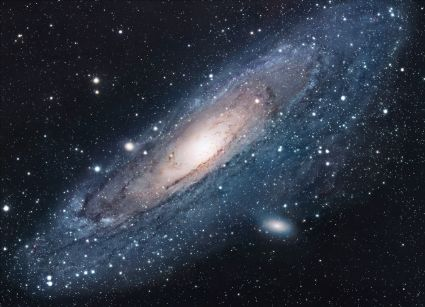
\includegraphics[scale=2]{img/universe.jpg}
        \caption{Isso é uma figura massa!}
        \label{fig:univerise}
    \end{figure}
\end{frame}
\begin{frame}[fragile]{Código Fonte: Figura}
    \begin{lstlisting}
    $\backslash$begin{figure}[h!]
    \centering
    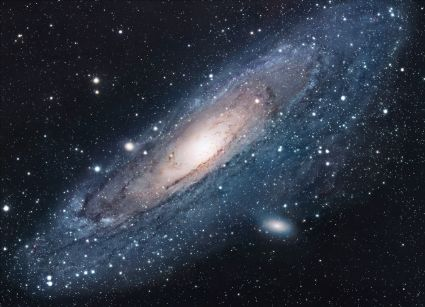
\includegraphics[scale=2]{img/universe.jpg}
    \caption{Isso é uma figura massa!}
    \label{fig:univerise}
    $\backslash$end{figure}
    \end{lstlisting}
\end{frame}

\begin{frame}{Recursos: Tabelas}
    \begin{table}[ht]
        \centering
        \begin{tabular}    {p{0.15\linewidth}p{0.15\linewidth}p{0.15\linewidth}p{0.15\linewidth}p{0.15\linewidth}}
            \hline
            coluna 1 & coluna 2 & coluna 3 & coluna 4 & coluna 5\\
            \hline
            1 & 2 & 3 & 4 & 5\\
            6 & 7 & 8 & 9& 10\\
            11 & 12 & 13 & 14 & 15\\
            16 & 17 & 18 & 19 & 20\\
            21 & 22 & 23 & 24 & 25\\
            \hline
        \end{tabular}
        \caption{Tabela de uma coluna num documento de várias colunas.}
    \end{table}
\end{frame}
\begin{frame}[fragile]{Código Fonte: Tabelas}
    \begin{lstlisting}
    \begin{table}[ht]
        \centering
        \begin{tabular}    {p{0.15\linewidth}p{0.15\linewidth}p{0.15\linewidth}p{0.15\linewidth}p{0.15\linewidth}}
            \hline
            coluna 1 & coluna 2 & coluna 3 & coluna 4 & coluna 5\\
            \hline
            1 & 2 & 3 & 4 & 5\\
            6 & 7 & 8 & 9& 10\\
            11 & 12 & 13 & 14 & 15\\
            16 & 17 & 18 & 19 & 20\\
            21 & 22 & 23 & 24 & 25\\
            \hline
        \end{tabular}
        \caption{Tabela de uma coluna num documento de várias colunas.}
    \end{table}
    \end{lstlisting}
\end{frame}


\begin{frame}{Recursos: Fórmulas}
    \begin{itemize}
            \item A famosa $e=mc^2$ de Albert Einstein !
            \item []
            \item Já essa: \[ e=\lim_{n \to \infty} \left(1+\frac{1}{n}\right)^n \] não é tão famosa assim...
            \item Imaginem essa:
            $$\left|{1\over N}\sum_{n=1}^N \gamma(u_n)-{1\over 2\pi}\int_0^{2\pi}\gamma(t){\rm d}t\right| \le {\varepsilon\over 3}.$$
    \end{itemize}
\end{frame}
\begin{frame}{Código Fonte: Fórmulas}
    \begin{itemize}
        \item Bom, melhor não ver agora...\\Acredite em mim, vai chegar a hora certa!
    \end{itemize}
\end{frame}
\begin{frame}[fragile]{Código Fonte: Fórmulas}
    \begin{itemize}
        \item Ok, vamos ver uma...
        \item []
        \begin{equation}
            \begin{array}{c}
                \underset{x\epsilon S^{n}}{\min}(f_{1}(x),\ldots,f_{k}(x));\quad
                \textrm{sujeito a }
                    \begin{cases}
                        g_{i}(x)\geq0\\
                        g_{l}(x)=0\\
                        x\epsilon S^{n}
                    \end{cases}
            \end{array}
            \label{eqn:1}
        \end{equation}
    \end{itemize}
    \begin{lstlisting}
    \begin{equation}
        \begin{array}{c}
            \underset{x\epsilon S^{n}}{\min}(f_{1}(x),\ldots,f_{k}(x));\quad
            \textrm{sujeito a }
            \begin{cases}
                g_{i}(x)\geq0\\
                g_{l}(x)=0\\
                x\epsilon S^{n}
            \end{cases}
        \end{array}
        \label{eqn:1}
    \end{equation}
    \end{lstlisting}
\end{frame}

\begin{frame}{Don't Panic!}
    \begin{alertblock}{Não entre em Pânico!}
        A maioria dos editores específicos de \LaTeX possuem interfaces gráficas para construções das tabelas, fórmulas, gráficos...\\
    \end{alertblock}
\end{frame}

%parâmetros: linguagem (shell, java, matlab, python, c, php) e arquivo

%\includecode[shell]{codigos/ola.sh}
%
%\includecode[matlab]{codigos/matlab.m}

%ou
% invocar os comandos \ansic, \java, \shell e colocar o código no próprio slide


\begin{frame}[fragile]{Recursos: Códigos}
    
    \includecode[ansic]{codigos/ola.c}	
    
    \ansic
    \begin{lstlisting}
    int main(void){
    printf("Ola mundo\n");
    return 0;
    }
    \end{lstlisting}
    \java
    
    \begin{lstlisting}
    public static voi main(String args[]){
    System.out.println("Ola mundo");
    }
    \end{lstlisting}	
    
\end{frame} 
\begin{frame}[fragile]{Código Fonte: Códigos}
    \begin{lstlisting}
    \begin{lstlisting}
    \includecode[ansic]{codigos/ola.c}	
    
    \ansic
    \begin{lstlisting}
        int main(void){
        printf("Ola mundo\n");
        return 0;
    }
    \ end{lstlisting}
    \end{lstlisting}

    \begin{lstlisting}
    \java
    \begin{lstlisting}
        public static voi main(String args[]){
        System.out.println("Ola mundo");
    }
    \ end{lstlisting}
    \end{lstlisting}
    
\end{frame} 

\section{Criando projetos em \LaTeX}
\begin{frame}{Praticando!}
    \begin{itemize}
        \item Comentários
        \item Macros "$\%$TODO"
        \item Indentação
        \item Separação de sílabas
        \item Iniciando nova linha
        \item Separação de arquivos
        \item Customizando texto
        \begin{itemize}
            \item \textit{itálico}
            \item \textbf{negrito}
            \item \underline{sublinhado}
            \item \textst{tachado}\footnote{Usa pacote específico}
        \end{itemize}
     \end{itemize}
\end{frame}

\begin{frame}{Praticando! Mergulhando fundo...}
    \begin{itemize}
        \item Nota de Rodapé
        \item Criando Epígrafes:
            \begin{itemize}
                \item \textit{epigraph}\footnote{Usa pacote específico}
                \item \textit{quote}
                \item \textit{description}
            \end{itemize}
        \item Criando Listas:
            \begin{itemize}
                \item \textit{itemize}
                \item \textit{enumerate}
                \item \textit{description}
            \end{itemize}
                
    \end{itemize}
\end{frame}

\begin{frame}{Praticando! Ao infinito e Além!}
    \begin{itemize}
        \item Criando Recursos Gráficos:
        \begin{itemize}
            \item Imagem
            \item Tabela
            \item Fórmulas
        \end{itemize}
        \item Criando Citações
        \begin{itemize}
            \item Seção
            \item Imagem
            \item Tabela
        \end{itemize}
        \item Criando novos comandos
        \item Criando referências 
        \item Citação de referências
        \item Alterando \textit{layouts}
        
    \end{itemize}
\end{frame} 


%Finalizando
\begin{frame}{Finalizando...}
    %Obrigado!
    %{Quero agradecer a todos por terem aguentado até aqui!
\end{frame} 
 
\begin{frame}{Referências}
 
\end{frame} 


\end{document}